\chapter{Methodology}

\label{chapter3}

% Intro
The chapter begins with the overall research design. Presents a brief overview of the methods used for the literature analysis and is followed by a description of the research type \textit{case study}, its justification and specifications. The methodology for selecting and conducting the interviews is described subsequently. The design frameworks on which the upcoming development is based are then presented in their original form. This includes the \acrfull{ssf}, which provided the overall process-oriented stage structure and the rough content orientation of the \acrfull{ssdr}, and the \acrfull{slmc}, which guided the development of the \acrfull{prc}. In order to adequately answer the two research questions building on these two main frameworks, they are complemented by a number of other guidelines and recommendations, which are briefly presented in the penultimate section of this chapter. A summary of the most important methodological and conceptual elements concludes this chapter.


\section{Research Design}

This work primarily applied an inductive perspective on quantitative analyses of conducted programs, projects and literature to synthesise best practices and guidelines. It also applied interpretive methods like interviews to gain new expert knowledge about the context and realities of the case study to build and apply new theory. Therefore, a combination of approaches will be reflected in a mixed-method approach which benefits of both, quantitative and qualitative data.

% lit analysis
The \textbf{background analysis} started with the review of the already established document database of the overarching \acrshort{eap} development and was subsequently extended. Broad concepts were used as a basis to lay a thematically large, yet steadily more specific foundation. For the in-depth analysis of previous \acrshort{cs} projects and further insights into the case study itself, grey and peer-reviewed literature was consulted. Grey literature, as academic literature specifically on Somalia was found to be generally scarce. The search was based on different combinations of keywords and their synonyms which could be derived from the underlying concepts and their respective specifications. Furthermore, in the course of the work, more specific literature and project suggestions were received from the project team and the interviewees. For the selection of CS projects, core areas of interest were formulated and derived from the thematic focus of the fundamental concepts and research aim. Therefore, the thematic focus was either on community-based participatory environmental or risk monitoring with regard to the issue of water, or on local projects using comparable methods. In the first case, geographical location, size or technical facilities were no exclusion criteria. Subsequently, the projects were tabulated and jointly evaluated manually, since the absolute number of projects finally selected was manageable without additional software.\newline
Available data about water sources in Somaliland was analysed via QGIS3. In total, five data sets about water sources in Somalia, a settlement layer and administrative boundaries were downloaded from the spatial \acrshort{fao}\acrshort{swalim} database (see Appendix \ref{AppendixA}). Three of the five water source data sets were different time instants of a single data series. All layers were projected to WGS84 / UTM zone 38N and subsequently clipped to the boundaries of Somaliland. The following analysis of the data was primarily exploratory, and extended with a basic statistical analysis.\newline 
In addition to the thematic focus on water-related issues, the methodically comparable practical implementation on the ground was investigated by analysing the already established \acrshort{cbs} program of the \acrshort{srcs}. This was done primarily by interviewing the responsible managers.

% Research Type
The \textbf{research type} that "allows in-depth, multi-faceted explorations of complex issues in their real-life settings" \autocite[1]{croweCaseStudyApproach2011} is the \textit{case research} or often just called \textit{case study}. This definition goes back to \textcite{yinCaseStudyResearch1984} and highlights the core strengths of this approach. The research type of the case study is particularly well suited for exploratory, rather than for descriptive or explanatory research, closely examining circumstances within a specific geographical area and context \autocite{zainalCaseStudyResearch2007}. Here, various quantitative and qualitative forms from both historical and real time data can be investigated and examined directly in its given context \autocite{fitzgeraldCaseStudiesResearch1999}. This allows for a detailed, multi-perspective and specific investigation of that particular topic of interest, which might not be given when examining the parts individually \autocite{pelzResearchMethodsSocial, zainalCaseStudyResearch2007}. Yet, case studies also comes with a number of trade-offs.\newline
More extreme critics see the case study method only as a loose 'story', which in the worse case is even connected to the scientist himself \autocite{fitzgeraldCaseStudiesResearch1999}. This criticism refers to the lack of rigour and "very little basis for scientific generalisation" \autocite[5]{zainalCaseStudyResearch2007} which can lead to low external validity \autocites{yinCaseStudyResearch1984}. The internal validity often remains weak due to no or poor experimental control complicating causal relationship testing and the multifaceted nature of case studies make it dependent on the researcher and prone to bias and some kind of subjectivity. Besides the internal and external validity, constructed validity and reliability need to be accounted for. Constructed validity refers to "the extent to which a study investigates what it claims to investigate" \autocite[3]{gibbertWhatPassesRigorous2008} so that "the researcher can correctly evaluate the studied concepts" \autocite[277]{ferreiraHowImproveValidity2020}. It can be addressed by establishing a clear chain of evidence and triangulation of perspectives and sources \autocite{gibbertWhatPassesRigorous2008}. Repeatability by other scientists using the same methodology to arrive at the same insights is termed 'reliability'. Repeatability refers therefore to the "absence of random error" \autocite[5]{gibbertWhatPassesRigorous2008} and can be enhanced by clear procedures and good documentation. Furthermore, case studies are frequently criticized for being excessively long, challenging to execute, and requiring significant documentation efforts \autocite{yinCaseStudyResearch1984}.
% justification case study
Since all research types have their advantages and disadvantages, it is primarily a weighing of these strengths and weaknesses that determines the choice of research type. The strength of the \textit{case study} make this research type ideal for addressing the aim of this study, as it allows for a holistic exploration and understanding of novel and under-researched areas within a "complex and dynamic context where it is difficult to isolate variables or where there are multiple, influencing variables" \autocites[2]{fitzgeraldCaseStudiesResearch1999}. Therefore, a case study is an excellent method not only to test theories but also to develop new theories and frameworks, as it is the aim of this study \autocite{pelzResearchMethodsSocial, zainalCaseStudyResearch2007}. Comparable studies, such as \textcite{asiimweUseInnovativeAffordable2011,frigerioHandsOnExperienceCrowdsourcing2018,kohlitzRuralDrinkingWater2020,minkmanCitizenScienceWater2015} and \textcite{weeserCitizenSciencePioneers2018a} have also successfully applied this research type.\newline
Along with the exploratory strategy, an iterative strategy was adopted, referring to the "visiting and revisiting [of] the data and connecting them with emerging insights, progressively leading to refined focus and understandings" \autocite[77]{srivastavaPracticalIterativeFramework2009}. Thereby, each interview or questionnaire was directly transcribed, coded, analysed and merged with previous insights. Along with the conducted literature analysis, newly acquired knowledge could thus be evaluated, triangulated, integrated and subsequently be used as a basis for further research and interviews allowing for deepening and refining of knowledge piece by piece.

% interviews
The selection of \textbf{interviewees} was based on a strategy of targeted expert sampling, i.e. a non-probability method that focused on reaching key informants and conducting expert interviews. This technique was employed as the expertise and experience of the individuals was crucial rather than focusing on broad, generalisable statements \autocite{pelzResearchMethodsSocial}. This method was further extended by adopting a snowball sampling approach which helped to identify further stakeholders and potential candidates.\newline
The target persons were primarily people who know the local context and are potential stakeholders in a possible implementation of the design in question. The first interview came about through existing contacts of the overarching EAP development project in which this work is embedded, and the interviewee was the project leader of the \acrshort{fbf} approach in the \acrshort{srcs} (I1). In the further course, the \acrshort{cbs} project manager of the Norwegian Red Cross (I2) and the \acrshort{cbs} manager on the Somali side (I3) were also interviewed. Between these two interviews, there was a second interview with the project manager of the \acrshort{srcs}' \acrshort{fbf} team (I1.2). More interviews with representatives of the Ministry of Water Resources, \acrshort{nadfor}, FAOSWALIM, \acrshort{brcis} and the technicians responsible for the NYSS platform were envisaged but could not be conducted. The interviews with the project leader on the \acrshort{srcs} side unfortunately had to be replaced by written questionnaires, as circumstances did not permit a personal interview. For the conversion of the interview guidelines into questionnaires, the recommendations of \textcite{harknessCCSGQuestionnaireDesign2016} were followed. The interviews and questionnaires themselves were semi-structured and mostly consisted of open ended questions to allow for the interviewee to give a free response as opposed to predefined answer options, see Appendix \ref{AppendixB}. Open-ended questions can facilitate more detailed answers, new insights and overall allow for an unlimited response in terms of scope and focus while they also complicate relevant information abstraction and following analysis \autocite{pelzResearchMethodsSocial}.\newline
The intelligent verbatim transcription of the interviews was facilitated by the newly developed neural net called Whisper \autocite{openaiIntroducingWhisper2022,openaiWhisper2023} and subsequently manually checked and corrected in MaxQDA 2022. For the further analysis, the recommendations of \textcite{radikerFocusedAnalysisQualitative2020} were followed. The coding strategy followed an inductive, open thematic manual coding approach. Codes were not strictly predefined, to be able to appropriately incorporate newly gained expertise, but only broadly categorized into the main themes of interest. More dedicated coding approaches based on e.g. the grounded theory or the hermeneutic analysis were not applied, as the given information was the focus of interest and not e.g. the identification of subjective constructs and underlying meaning \autocite{pelzResearchMethodsSocial}. Nonetheless, based on the criticism on positivism, provided information was not taken as unbiased and objective but interpreted in the context of its perspective.

\section{Design Frameworks}\label{sec:design_framework}

The design of the roadmap for community-based water source monitoring was particularly guided by the framework of \textcite{fraislCitizenScienceEnvironmental2022}. This framework was chosen as it is very up-to-date, incorporates many guidelines and best practices, and structures them in an efficient and process-oriented way, with a focus on practical applicability. It covers the entire life cycle of a Citizen Science project in its six phases in an iterative way, starting with problem assessment and finishing with evaluation procedures. However, the focus is on ecological and environmental projects, which necessitated a thorough revision of the content.\newline
The framework was tailored to the study area and research aim by adapting and extending it with other thematic and context related experiences and guidances. Stage 1 was extended by context specific topics and Stage 2 majorly expanded with a feasibility assessment based on the \textcite{ifrcCommunityBasedSurveillanceGuiding2017}. The biggest expansion, however, came from the third stage onwards. From here on, the \acrshort{ssf} was additionally accompanied by a self developed \acrfull{prc}. The \acrshort{prc} was primarily structured along the \acrlong{slmc} design pattern and incorporates the recommendations of several other guidelines as well as gained knowledge through the literature review and the project analysis. This fundamentally expanded the process-oriented \acrshort{ssf} structure with a requirement and dependency focussed skeleton in order to further reduce cognitive overload, see section \ref{sec:prc}.\newline
The original version of the utilized frameworks, the \acrshort{ssf} and the \acrshort{slmc}, followed by a section about several other \acrshort{cs} guidelines will be presented in this section. This lays the foundation for the results related to the first research question in sections \ref{sec:ssdr} and \ref{sec:prc} and enables further application in section \ref{sec:f_a} to address the second research question.

\subsection{Six-Stage-Framework}\label{subsec:ssf}

In their work, \textcite{fraislCitizenScienceEnvironmental2022} pull information from all kinds of \acrshort{cs} programmes, projects and scientific guidance. Although thematically focused on projects in the field of ecology and environmental sciences, the underlying principles described here are also applied in a variety of thematically differently oriented projects \autocite{fraislCitizenScienceEnvironmental2022}. The developed \acrfull{ssf} concentrates on the participation level (1) crowdsourcing and (2) distributed intelligence. On these levels, citizens are primarily contributors and partly asked to interpret the sensed information. This was outlined in chapter \ref{sec:cs}. All six stages are interconnected and should all be considered throughout the project to incorporate new information, feedback and lessons learned \autocite{fraislCitizenScienceEnvironmental2022}. An overview of the \textit{citizen science project life cycle} can be seen in figure \ref{fig:meth_ssf}.

\begin{figure}[!htp]
    \centering
    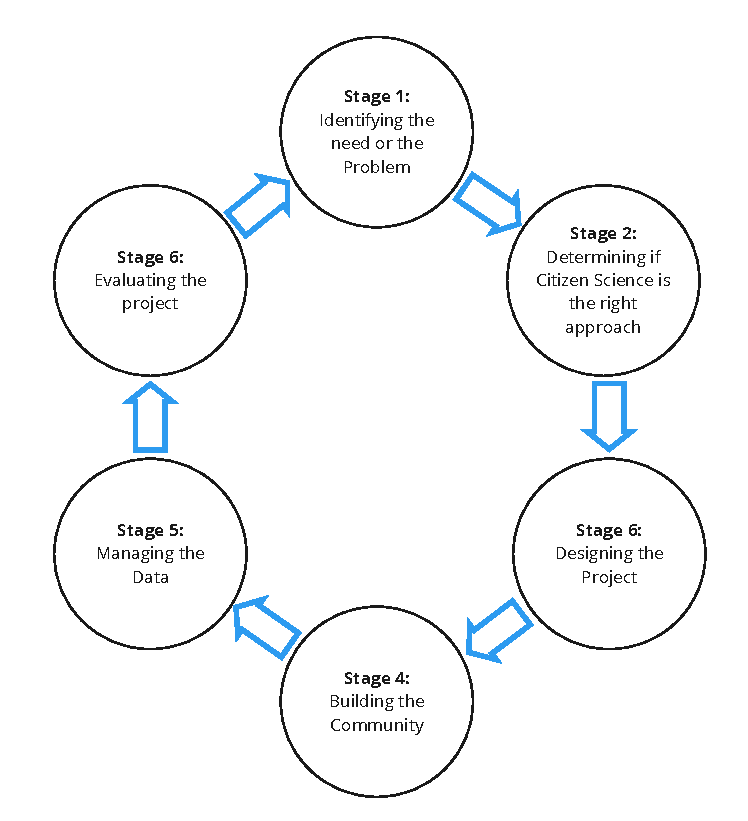
\includegraphics[width=0.7\textwidth]{figures/2023_MA_methods_ssf_original.pdf}
    \decoRule
    \caption[The Six Stages Framework]{The Six Stages Framework for designing a citizen science project in ecology and environmental sciences. Source: \autocite[4]{fraislCitizenScienceEnvironmental2022}}
    \label{fig:meth_ssf}
\end{figure}

In stage 1 the overall need and problems are identified and their boundaries defined. This includes the gathering of potential solutions, limitations and the formulation of research questions. Stage 2 closely examines the potential application of \acrshort{cs} in the identified boundaries. The focus is on the fruitfulness of the involvement of participants to reach the formulated objectives and answer the research questions. This may be related to many project specifications, e.g. temporal and spatial scale, required expertise and intended target groups. As the second major consideration for the reasonable integration of \acrshort{cs} participants, \textcite{fraislCitizenScienceEnvironmental2022} note, that the project need to benefit the participants by "addressing their needs or fostering new skill and expertise" (p.2). After problems, needs and applicability are addressed, the objectives and aims of the project need to be defined in detail together with the prospective stakeholders in stage 3. In addition to the main objectives, secondary objectives such as awareness and knowledge building as well as its transfer could also be pursued. Establishing an initial foundation for concerns of privacy and ethics, data storage and analysis, selection of methods and training strategies as well as means of communication and respective instruments is also part of this stage. Furthermore, the tasks of the participants need to be defined in detail, also including any benefits and safety considerations. Stage 4 is concerned with the building of the community by identifying participants motivations, education levels and other demographic information as well as issues of acknowledgments, feedback and sustaining participation. Planning of data management in terms of collection, storage, \acrfull{qc} and \acrfull{qa}, analysis and privacy and security are highlighted in stage 5. Although evaluation is the main theme of stage 6, it is seen more as an ongoing effort that is recommended throughout the project to allow for feedback and improvement at each stage.

\subsection{Seven-Layer Model of Collaboration}\label{subsec:slmc}

The design pattern of the \acrshort{slmc} was utilized to develop a new requirement focussed catalogue to enhance the applicability of the \acrshort{ssf} from stage three \textit{designing the project} and onward to better handle and structure the high complexity and interdependences. The \acrshort{slmc} was specifically designed to reduce cognitive (over-)load for the design of a complex, interrelated project in a social-technical context. It does so, by separating concerns at design time into seven layers and corresponding methods and techniques. These, as presented by \textcite{briggsSevenLayerModelCollaboration2009}, are primarily aimed at the collaboration of groups, but the overall pattern can be preserved when applied to designs in other contexts \autocite{diggelenGroundedDesignDesign2009}. Therefore, the following explanations of the individual layers, their methods and techniques are adapted to this work, while maintaining the general pattern, see \textcite{briggsSevenLayerModelCollaboration2009}. The seven, slightly adjusted layers are: Goals, Products, Activities, Methods, Techniques, Tools and Scripts, see figure \ref{fig:meth_slmc}.\newline
\pagebreak
\begin{wrapfigure}{r}{0.25\textwidth}
    \vspace{20pt}
    \centering
    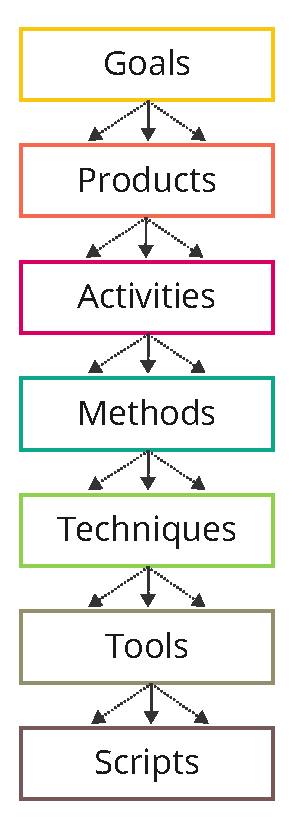
\includegraphics[width=0.2\textwidth]{figures/2023_MA_methods_slmc_vertical_arrows.pdf}
    \rule{0.25\textwidth}{0.1pt}
    \caption[The Seven Layer Model of Collaboration]{The Seven Layer Model of Collaboration. Source: Own representation based on \textcite{briggsSevenLayerModelCollaboration2009}}
    \label{fig:meth_slmc}
    \vspace{20pt}
\end{wrapfigure}
The layers are ordered hierarchically with Goals being the top-most layer. Changes made in one layer, may need to be accounted for in the lower, but not necessarily in the upper layers. The \textit{Goal-Layer} incorporates all overarching goals and objectives of the project. The \textit{Products-Layer} sums up all tangible or intangible components or outcomes that are necessary to achieve the formulated targets in the \textit{Goal-Layer}. The required activities that yield these products, are grouped in the \textit{Activities-Layer}. These activities formulate what needs to be done in order to create the necessary products and can have sub-products and sub-activities of their own. The fourth \textit{Method-Layer} is the most different from the original, as it does not deal with the procedures of collaboration but with the methods used in the activities. The \textit{Techniques-Layer} specifies the involved techniques and practices and the \textit{Tools-Layer} summarises all relevant artifacts or apparatus used. The final procedures are described in detail and defined in the bottommost layer, the \textit{Script-Layer}. Further concerns, interactions and justifications between and for each layer are extensively described by \textcite{briggsSevenLayerModelCollaboration2009} and while there is a lot of value in these remarks, the thematic adaptations and focus of this work make further exploration in this context obsolete. Nonetheless, interested readers are invited for further independent exploration. In this work, emphasis is given to the top three layers, the \textit{Goal-, Products-, and Activities-Layer} as these could be handled in terms of the level of detail without having to be on site.

\subsection{Citizen Guidelines \& Recommendations}

This section presents some further guidelines and recommendations that have been used to complement and adapt the framework described above to the objective and context of this work. These recommendations, frameworks and guidelines for \acrlong{cs} projects have become numerous and thematically wide-ranging. Networks and programmes of researchers and practitioners covering all or parts of the stages proposed by the \acrshort{ssf} are spatially widespread at the global level and include a variety of regional, national or global application levels. Some examples of such networks and programmes are government programmes such as the US-run \href{https://www.citizenscience.gov/}{citizenscience.gov} website or the EU platform \href{https://eu-citizen.science/}{eu-citizen.science}, support platforms such as \href{https://citsci.org/}{CitSci} and the \href{https://citizenscience.ch/en/}{Citizen Science Center Zurich} as well as regionally focused associations like \href{http://cienciaparticipativa.net/la-ricap/}{La Red Iberoamericana de Ciencia Participativa (RICAP)}, \href{https://citizenscience.asia/}{CitizenScience.Asia} and the \href{https://www.usiu.ac.ke/citsci-africa-association/}{Citizen Science Africa Association}.\newline
Besides these knowledge-hubs, a vast variety of different scientific and and grey literature exists. \Textcite{fraislCitizenScienceEnvironmental2022} and \textcite{westonCommunityBasedWaterMonitoring2015} have each listed and summarized many recommendations and \textcite{garciaFindingWhatYou2021} even created a guide to citizen science guidelines.\newline
Furthermore, \textcite{minkmanCitizenScienceWater2015} derived a set of six potential goals which could be addressed through \acrlong{cs} in water management namely (a) awareness raising, (b) public education, (c) policy development, (d) method improvements, (e) knowledge building, and (f) management improvements. The demarcation between the individual goals can be fluid and is not rigidly predetermined. Each \acrshort{cs} project can address multiple of these goals and with varying emphasis. These goals were derived in cooperation with water management authorities in the Netherlands and concentrate on objectives that can be implemented in practice.\newline
Although the overall objective of this work was already defined, all these six goals by \textcite{minkmanCitizenScienceWater2015}were chosen as a starting point for further exploratory analysis in order not to overlook potentially useful secondary goals. These six goals formed the first layer of the \acrshort{slmc} in the development of the \acrshort{prc}. Further emphasis was given to the findings of the \acrshort{brcis} network and \acrshort{ifrc}'s \acrshort{cbs} and \acrshort{fbf} guidelines, manuals and recommendations. Further information of the above-mentioned projects, programmes, associations and others was integrated by extracting the key findings and guidance from the respective papers and projects, categorising them along the stages and then integrating them into the stages of the newly developed framework.

% possibly include something like
% and a collection of those guidelines can be seen in Table XYZ
% BRCiS learning, Minkman guidelines and so on.. + ESCA 10 guidelines and characteristics + all guidelines listed by weston 2015

\section{Method Summary}

This chapter presented the research design and methods used, as well as the framework conditions that guided the design and application of the study. This work was embedded in a primarily inductive research design of an exploratory, iterative case study, and adopted a mixed-method approach with data and document analysis as well as expert interviews. The development of the new community-based water source monitoring framework was primarily based on two frameworks, the \acrfull{ssf} and the \acrfull{slmc}. The \acrshort{ssf} primarily provided the structural basis and content orientation for the development of the process-oriented \acrlong{ssdr} and the \acrshort{slmc} gave orientation to the creation of the \acrlong{prc}. Moreover, several other guidelines and recommendations were outlined which were incorporated to complement and adapt the two main frameworks to this research's aim and context. The expert interviews conducted subsequently enabled the application of this new and adapted framework to create the implementation roadmap for Somaliland.
